% -*- root: ../thesis.tex -*-
%!TEX root = ../thesis.tex

% ******************************* Thesis Chapter 1 ****************************

% the code below specifies where the figures are stored
\ifpdf
    \graphicspath{{chapters/1_introduction/figures/}}
\else
    \graphicspath{{1_introduction/figures/EPS/}{1_introduction/figures/}}
\fi
% ----------------------------------------------------------------------
%: ----------------------- introduction content ----------------------- 
% ----------------------------------------------------------------------

\ac{ML} is today a wide field of research with plenty of successful applications, in particular with fields such as computer vision, natural language processing or reinforcement learning \needcite.
A particular field of interest is \textit{probabilistic} machine learning.
When one starts to consider all quantities of interest as random variables, paradigms and tools from statistics can be used, and stronger analysis can be derived.
% Probabilistic models provide uncertainties to results and
It does not only produce more complete and rich results but also helps connect with more standard sciences such as physics or climatology where using statistical tools is standard practice.

\section{Bayesian Machine Learning}

Some real-world problems have critical requirements.
For example when decision-making is involved, probability guarantees for predictions and meaningful interpretable models are essential.
The Bayesian framework brings both these aspects by working with \textit{random variables} defined by \textit{probability distributions} instead of point estimates.
For a given probabilistic model, by setting a \textit{prior distribution} over the parameters of interest, the \textit{posterior distribution} represents the updated belief we have about our model after observing some data.
This allows modelling uncertainty in a principled way and prevents overfitting in the low-data regime.\needcite
A typical example is in medicine, where data is scarce, but the predictive outcome can have a dramatic effect (diagnosis, prognosis, etc...).
Providing uncertainties is the only way to help the practitioner make a decision given the model predictions.

Generally, Bayesian models come with a higher computational cost: a probability distribution needs more parameters as it contains more information than a single point, calculus with random variable is a complex science and finding analytical solutions happens almost exclusively for trivial models.
To be able to work with more complex models, a lot of research focus on approximation algorithms, which will provide an incorrect solution that can be provably useful.
This is the general scope of \textit{approximate Bayesian inference}.

The research goes in many directions, but some main ones are: How to compute the most accurate posterior approximation as efficiently as possible? How can it be made scalable with larger amount of data and/or parameters? What are the guarantees of such algorithms?
The works presented in this thesis aim at answering partially these questions for some given setups, in particular through the lens of model representation.

\section{The underestimated power of representations choices}

% \begin{itemize}
%     \item Different representation lead to very different results, efficiency etc.
%     \item Mention existing approaches
% \end{itemize}
The leading thread of this thesis is \textit{model representation}, alternatively called \textit{model parameterization}, and its use for solving problems more efficiently and faster without compromising prediction quality.

When defining probabilistic models, one needs to define relations between variables (observed and latent) and choose appropriate distributions to represent those.
Some modelling choices are equivalent conceptually but have drastic differences when it comes to inference.
A neat example, presented in \citet{gorinovaAutomaticReparameterisationProbabilistic2020}, is the so-called Neal's funnel.
There are two equivalent representations, called centered and non-centered, shown respectively in Figure~\ref{fig:neals_centered} and~\ref{fig:neals_noncentered}, where one leads to an inference nightmare while the other is a nice and easy isotropic Gaussian distribution.

\begin{minipage}{0.5\textwidth}
    \centering
    \begin{align}
        \begin{aligned}
            z \sim&\; \mathcal{N}(0, 3)\\
            x \sim&\; \mathcal{N}(0, \exp(z/2))
        \end{aligned}
    \end{align}
    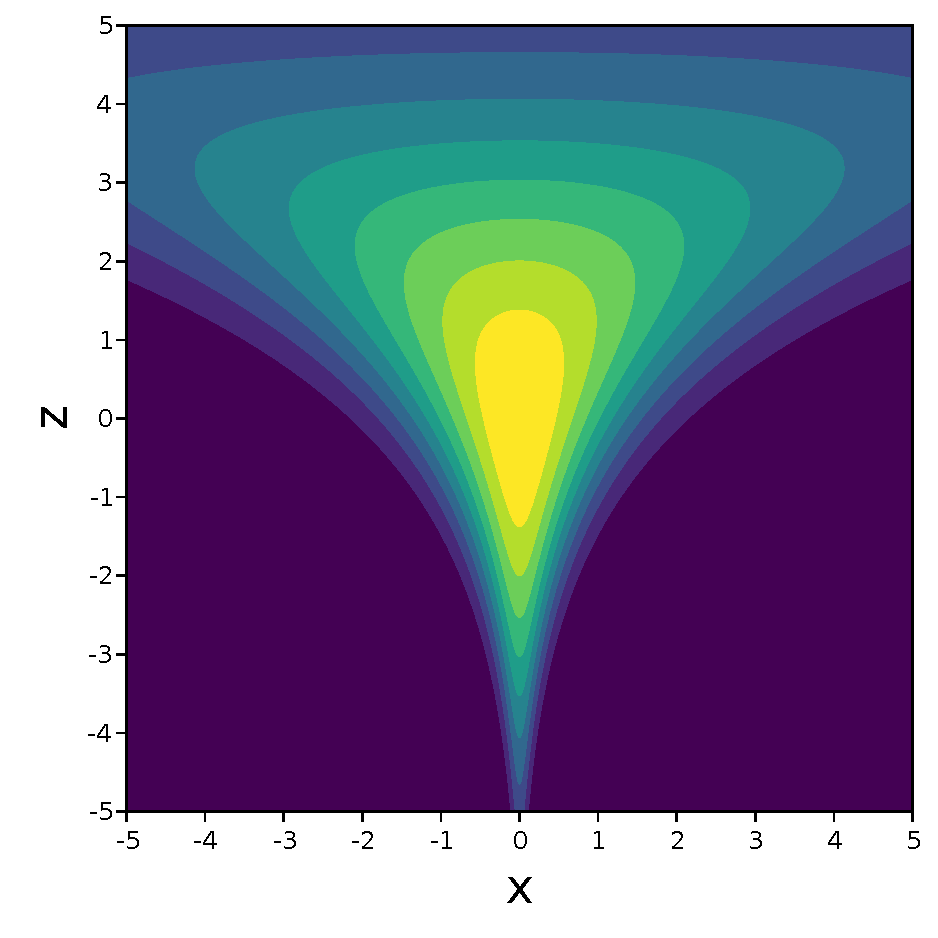
\includegraphics[width=\textwidth]{./chapters/1_introduction/figures/neals_funnel_centered.pdf}
    \captionof{figure}{Neal's funnel - Centered representation}
    \label{fig:neals_centered}
\end{minipage}
\begin{minipage}{0.5\textwidth}
    \centering
    \begin{align}
        \begin{aligned}
            \tilde{z} \sim&\; \mathcal{N}(0, 1),\quad z = 3\tilde{z}\\
            \tilde{x} \sim&\; \mathcal{N}(0, 1),\quad x = \exp(z/2)\tilde{x}
        \end{aligned}
    \end{align}
    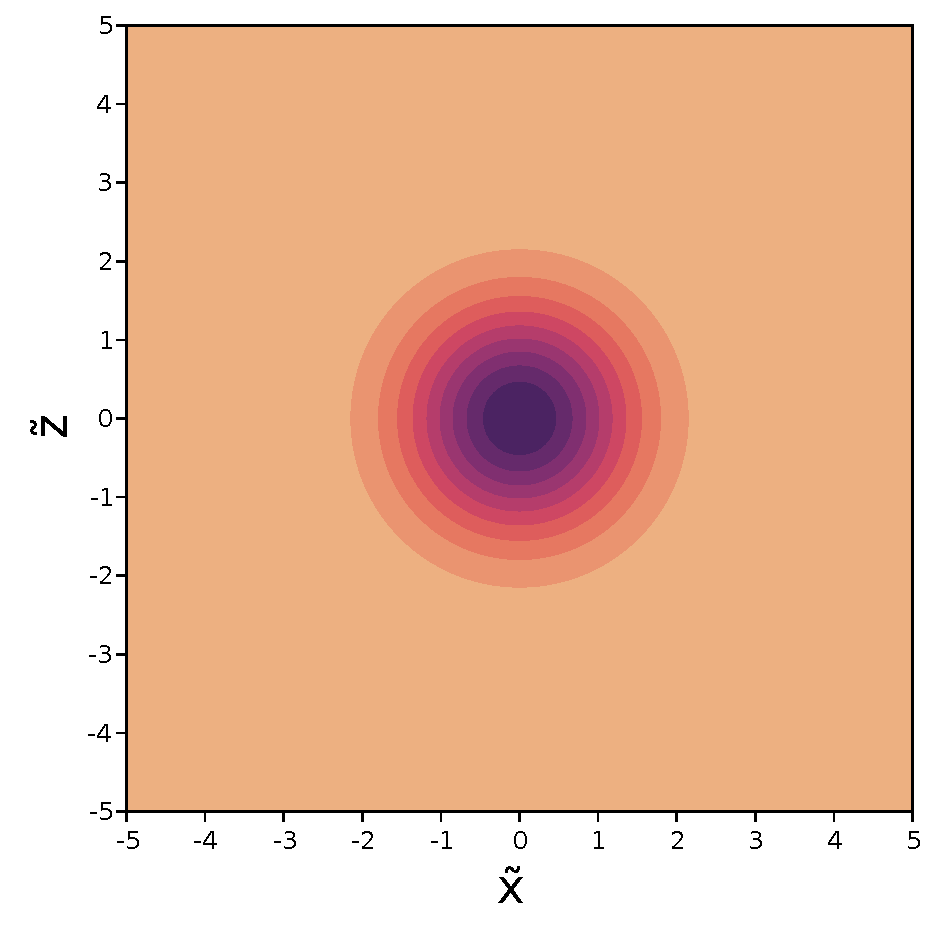
\includegraphics[width=\textwidth]{./chapters/1_introduction/figures/neals_funnel_non_centered.pdf}
    \captionof{figure}{Neal's funnel - Non-centered representation}
    \label{fig:neals_noncentered}
\end{minipage}
\vspace{0.5cm}

While both parameterizations are one and the same, working with $p(\tilde{x},\tilde{z})$ is obviously simpler.
An analogy in physics would be of how easier it is to work with spherical coordinates instead of Euclidean ones for electrodynamics. 

Working on model representations is often underestimated and are mostly considered "tricks".
For example, when working with \acf{GPs}, it is preferable to use the so-called "whitened" representation, which corresponds to our non-centered representation in of the Neal's funnel.
The different works in this thesis show that finding better representations can confidently make inference not only easier, but also faster and more importantly much more stable. 
A first part will focus on how the likelihood can be represented as (hierarchical) mixtures and how the most basic inference methods can be then used.
Defined later in Section \ref{sec:scale-mixtures}, variables that can be rewritten as scale-mixtures have a lot of advantages and interesting properties.
Writing them explicitly as mixtures, i.e. by augmenting the model with a new latent variable, makes inference considerably easier while keeping the original model intact.
This augmentation procedure brings the counter-intuitive view that adding more variables actually \textit{simplifies} the problem.
The last work of the thesis will focus on the representation of the approximation, by using a non-conventional particle approach, computational bottlenecks can be lifted and more flexibility on the result. 


\section{Gaussian Processes}

The forementioned works apply to most probabilistic models, however a strong focus is made on Gaussian based models, and more particularly \acf{GPs}.
A \ac{GP} is a strong non-parametric tool to approximate functions using probabilistic methods.
They used to be reserved to Gaussian regression problems, like the original \textit{kriging problem} \cite{cressie1990origins}, but they can also be used as latent function for more complex problems like classification, ordinal regression and more.
Compared to other general function approximators like neural networks, they have the advantage to provide uncertainty on the prediction they make.
Their non-parametric nature naturally avoids over-parametrization: while modern neural networks have billions of parameters to optimize, \ac{GPs} only depend on a mean function and a kernel function.
Most importantly, as their name suggest, they are based on Gaussian distributions, making them the best candidates for the presented work on augmentation.
A full technical introduction to basic \ac{GPs} and its extensions is given in Section~\ref{sec:gps}.

\section{Open-source projects}

All the works presented in this thesis as well as additional tools are backed-up by user-friendly packages in Julia \cite{Julia-2017}.
Throughout my time as a Ph.D. student I have developed numerous Julia packages and in particular was involved in the \href{https://github.com/JuliaGaussianProcesses}{JuliaGaussianProcesses organisation} to develop a flexible, efficient and easy-to-use framework to work with \ac{GPs} from the very low-end to high-end interfaces through a series of packages: \href{https://github.com/JuliaGaussianProcesses/KernelFunctions.jl}{KernelFunctions.jl}~\cite{theo_galy_fajou_2022_6246597}, \href{https://github.com/JuliaGaussianProcesses/AbstractGPs.jl}{AbstractGPs.jl}~\cite{david_widmann_2022_5939997}, \href{https://github.com/JuliaGaussianProcesses/ApproximateGPs.jl}{ApproximateGPs.jl} and \href{https://github.com/JuliaGaussianProcesses/GPLikelihoods.jl}{GPLikelihoods.jl}.
The particular strength of our work is the one-to-one mapping between theory and code.
For example to define the posterior for some given data, the code looks like:
\begin{minted}[breaklines,escapeinside=||,mathescape=true, numbersep=3pt, gobble=2, frame=lines, fontsize=\small, framesep=2mm]{julia}
    f = GP(mean_prior, kernel) # define an infinite-dimensional prior
    fx = f(X, noise) # create a realization on the data X
    fpost = posterior(fx, y) # Create the posterior given the observations y
\end{minted}
Here, each computational object represents exactly its mathematical equivalent.

The work of this thesis is represented as well with the package \href{https://github.com/JuliaGaussianProcesses/AugmentedGPLikelihoods.jl}{AugmentedGPLikelihoods.jl}, which provide all the necessary tools to work with augmentations.
Julia has the advantage to have an extremely strong interoperability capacity.
This allows to use the augmentation work on specific implementation of \ac{GPs} such as temporal \ac{GPs} with a concrete example given in \href{https://github.com/JuliaGaussianProcesses/TemporalGPs.jl}{TemporalGPs.jl} (see examples/augmented\_inference.jl).

Independently, I also developed \href{https://github.com/theogf/AugmentedGaussianProcesses.jl}{AugmentedGaussianProcesses.jl}~\cite{theo_galy_fajou_2021_5728215} as a stand-alone \ac{GP} package providing the augmentations techniques presented in the thesis, additional likelihoods and standard inference approaches.

\section{Thesis Outline}

This thesis is constructed as follows:
\begin{itemize}
    \item Chapter~\ref{ch:background} will introduce in details all the common concepts to Bayesian inference and \ac{GPs}.
          This background is generally introduced in each of the published articles, but this chapter allows going more in-depth in the background theory.
          Bayesian inference will be properly introduced with a focus on variational inference and sampling.
    \item Chapter~\ref{ch:classification} introduces the paper \textit{Efficient Gaussian Process Classification Using P\`olya-Gamma Data Augmentation}, which was the first step of this thesis using augmentations to improve and scale up inference.
    \item Chapter~\ref{ch:multiclass} introduced the paper \textit{Multi-Class Gaussian Process Classification Made Conjugate: Efficient Inference via Data Augmentation}.
          This paper brings new concepts of augmentation to a much more complex problem: multi-class classification.
    \item Chapter~\ref{ch:general} introduces the paper \textit{Automated Augmented Conjugate Inference for Non-conjugate Gaussian Process Models}.
          This work was the first generalization of one type of augmentation and allowed to get a much better understanding of these concepts.
    % \item Chapter \ref{ch:chapter6} introduces the draft of the paper \textit{\com{fill in}} currently under review.
    % This paper solves of the issues rising when using scalable \ac{GPs} models by using sampling and other techniques.
    \item Chapter~\ref{ch:gpf} introduces the paper \textit{Flexible and Efficient Inference with Particles for the Variational Gaussian Approximation } a completely different way of performing variational inference with Gaussian distribution by using a continuous flows and particles.
    \item Chapter~\ref{ch:discussion} introduces multiple discussions about the different works presented as well as some concrete outlooks on how new models and new generalizations could be explored.
    \item Chapter~\ref{ch:conclusion} finished this thesis with a general conclusion.
    \item Two additional workshop papers which do not fit the narrative of this thesis have been added in the Appendix~\ref{appendix:worshoppapers}

    For all papers, the contribution will be detailed using a simplified view of the \href{https://mdpi-res.com/data/contributor-role-instruction.pdf}{Contributor Roles Taxonomy} (CReditT).

\end{itemize}

